% !TeX root = ../main-presentation.tex
\begin{frame}
    \frametitle{What came before}

    \pause
    \centering
    \LARGE
    String graphs
    \raisebox{-2em}{
        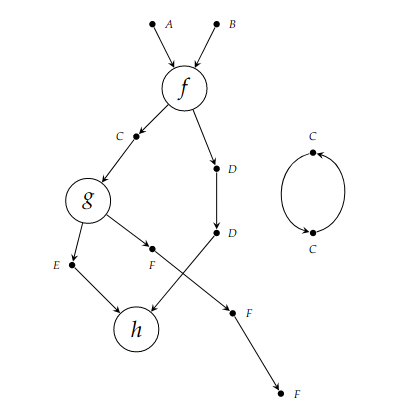
\includegraphics[width=0.2\textwidth]{string-graphs}
    }

    \pause
    \normalsize
    \vspace{1em}
    Dixon, Kissinger

    
\includegraphics[width=0.15\textwidth]{dixon}
    
\includegraphics[width=0.15\textwidth]{kissinger}

\end{frame}

\begin{frame}
    \frametitle{What came before}

    \pause
    \centering
    \LARGE
    Hypergraphs
    \quad
    \raisebox{-1.5em}{
        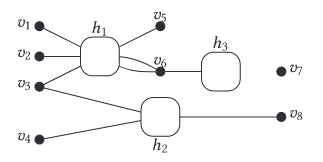
\includegraphics[width=0.3\textwidth]{hypergraphs}
    }

    \pause
    \normalsize
    \vspace{1em}
    Bonchi, Gadduchi, Kissinger, Sobocinski, Zanasi

    \hypergraphpeople

\end{frame}

\begin{frame}
    \frametitle{The hyper kind of graph}

    \centering
    \dsptikzfig{graphs/example}

\end{frame}

\begin{frame}
    \frametitle{The hyper kind of (interfaced) graph}

    \centering
    \dsptikzfig{graphs/example-cospan}

\end{frame}

\begin{frame}
    \frametitle{Terms to graphs}

    \centering
    \LARGE

    Goal:

    Interpret \alert{string diagrams} as \alert{cospans of hypergraphs}

    \vspace{1em}
    \pause

    But which hypergraphs?

\end{frame}

\begin{frame}
    \frametitle{Hyp}



\end{frame}

\begin{frame}
    \frametitle{Feeling special}

    \centering

    \LARGE
    Which terms correspond to cospans of hypergraphs?

    \pause

    \normalsize
    Special commutative Frobenius structure

    \pause
    \normalsize
    \vspace{1em}
    \dsptikzfig{strings/structure/monoid/init}[white]
    \dsptikzfig{strings/structure/comonoid/copy}[white]
    \dsptikzfig{strings/structure/monoid/merge}[white]
    \dsptikzfig{strings/structure/comonoid/discard}[white]
    \pause
    \vspace{1em}

    Any category with this structure is \alert{self-dual compact closed}
    \pause
    \[
        \dsptikzfig{strings/compact-closed/cup}
        :=
        \dsptikzfig{strings/structure/monoid/init}[white]
        \scalebox{1.5}{\(\seq\)}
        \dsptikzfig{strings/structure/comonoid/copy}[white]
        \qquad
        \dsptikzfig{strings/compact-closed/cap}
        :=
        \dsptikzfig{strings/structure/monoid/merge}[white]
        \scalebox{1.5}{\(\seq\)}
        \dsptikzfig{strings/structure/comonoid/discard}[white]
    \]

\end{frame}


\begin{frame}
    \frametitle{Feeling special graphs}

    \centering

    \begin{minipage}{0.45\textwidth}
        \begin{center}
            isomorphism class of hypergraphs

            \vspace{1em}

            \scalebox{0.625}{\dsptikzfig{graphs/example-frobenius-cospan}}
        \end{center}
    \end{minipage}
    \quad
    \raisebox{-1em}{\(\leftrightarrow\)}
    \pause
    \begin{minipage}{0.45\textwidth}
        \begin{center}
            Frobenius term

            \vspace{1em}

            \dsptikzfig{graphs/example-frobenius-term}
        \end{center}
    \end{minipage}

    \vspace{1em}
    \pause
    \normalsize
    \scalebox{0.75}{\hypergraphpeople}

    \vspace{1em}
    \Large
    \pause

    So vanilla hypergraphs are \alert{not restrictive enough}.

\end{frame}

\begin{frame}
    \frametitle{A bit too special}

    \centering

    What hypergraphs correspond to \alert{symmetric monoidal} terms?

    \vspace{1em}

    \begin{minipage}{0.45\textwidth}
        \begin{center}
            `monogamous acyclic' hypergraphs

            \vspace{1em}

            \scalebox{0.625}{\dsptikzfig{graphs/example-monogamous-acyclic}}
        \end{center}
    \end{minipage}
    \quad
    \raisebox{-1em}{\(\leftrightarrow\)}
    \pause
    \begin{minipage}{0.45\textwidth}
        \begin{center}
            symmetric monoidal term

            \vspace{1em}

            \dsptikzfig{graphs/example-smc-term}
        \end{center}
    \end{minipage}

    \vspace{1em}
    \pause
    \normalsize
    \scalebox{0.75}{\hypergraphpeople}

    \vspace{0.5em}
    \Large
    \pause

    Monogamous acyclic hypergraphs are \alert{too restrictive}.

\end{frame}

\begin{frame}
    \frametitle{Frobenius to traced comonoid}

    \centering
    \LARGE
    Traced comonoid is `almost' Frobenius...


\end{frame}

\begin{frame}
    \frametitle{<title>}

    Partial left-monogamy

\end{frame}

\begin{frame}
    \frametitle{<title>}

    Traced comonoid terms
    \(\leftrightarrow\)
    Partial left-monogamous hypergraphs

    
\includegraphics[width=0.15\textwidth]{ghica}
    
\includegraphics[width=0.15\textwidth]{me}

\end{frame}